\chapter{Mechanical Power Transmission}\label{ch:transmission}

\begin{tipbox}[When to Read This Chapter]
\textbf{Sprint~2--3}: Read the motor-to-load matching section when sizing your drivetrain. \textbf{Sprint~3 (CDR)}: Use the transmission components quick-reference table to specify parts for your BOM. The 3D-printed gear section applies if you are prototyping custom gears.
\end{tipbox}


\vspace{1em}

Power transmission converts motor output (torque and speed) into the motion your system needs. Every element, belt, chain, gear, shaft, linkage, lead screw, trades speed for torque (or vice versa), and every one introduces losses. Selecting the right transmission is the bridge between your electrical power budget and the mechanical work your system must perform.

\vspace{1em}

\section{Fundamental Relationships}
Three equations govern all power transmission:
\begin{align}
\text{Gear ratio:} \quad GR &= N_2/N_1 = \omega_1/\omega_2 = \tau_2/\tau_1 \\
\text{Power:} \quad P &= \tau \times \omega \\
\text{Efficiency:} \quad \eta &= P_{\text{out}}/P_{\text{in}}
\end{align}
\textbf{Speed down $\to$ torque up} by the gear ratio; power constant minus losses. Multi-stage efficiency compounds: $0.95^3 = 85.7\%$.

\section{Belt and Pulley Drives}
\subsection{V-Belts}
Wedge cross-section grips by friction. Allows slip (protects downstream). 90--95\% efficient. Requires tension adjustment.

\subsection{Timing Belts (Synchronous)}
Toothed belts mesh with toothed pulleys; no slip, positive drive. 97--99\% efficient.

\begin{tipbox}[GT2 Timing Belts for Student Projects]
GT2 profile (2\,mm pitch, 6\,mm width) is the standard for student projects, 3D printers, and hobby CNC. \$3--8/meter on Amazon. Pulleys 16--60 tooth for \$2--5. Always use flanged pulleys to prevent belt tracking.
\end{tipbox}

\subsection{Flat and Round Belts}
Flat belts on crowned pulleys for long center distances. Round belts (O-ring) for low-load, compact drives.

\section{Chain Drives}
Roller chain: positive engagement, 95--98\% efficient, high loads and shock tolerance. \#25 (1/4\,in pitch) for student projects. Minimum 17 teeth on small sprocket.

\begin{tipbox}[Chain Requires Lubrication]
Dry chain wears at $10\times$ the rate of lubricated chain. Apply chain lubricant (not WD-40) every 20--50 operating hours. A worn chain skips teeth; sudden and dangerous.
\end{tipbox}

\section{Gear Trains\index{gear train}}

\begin{figure}[htbp]\centering
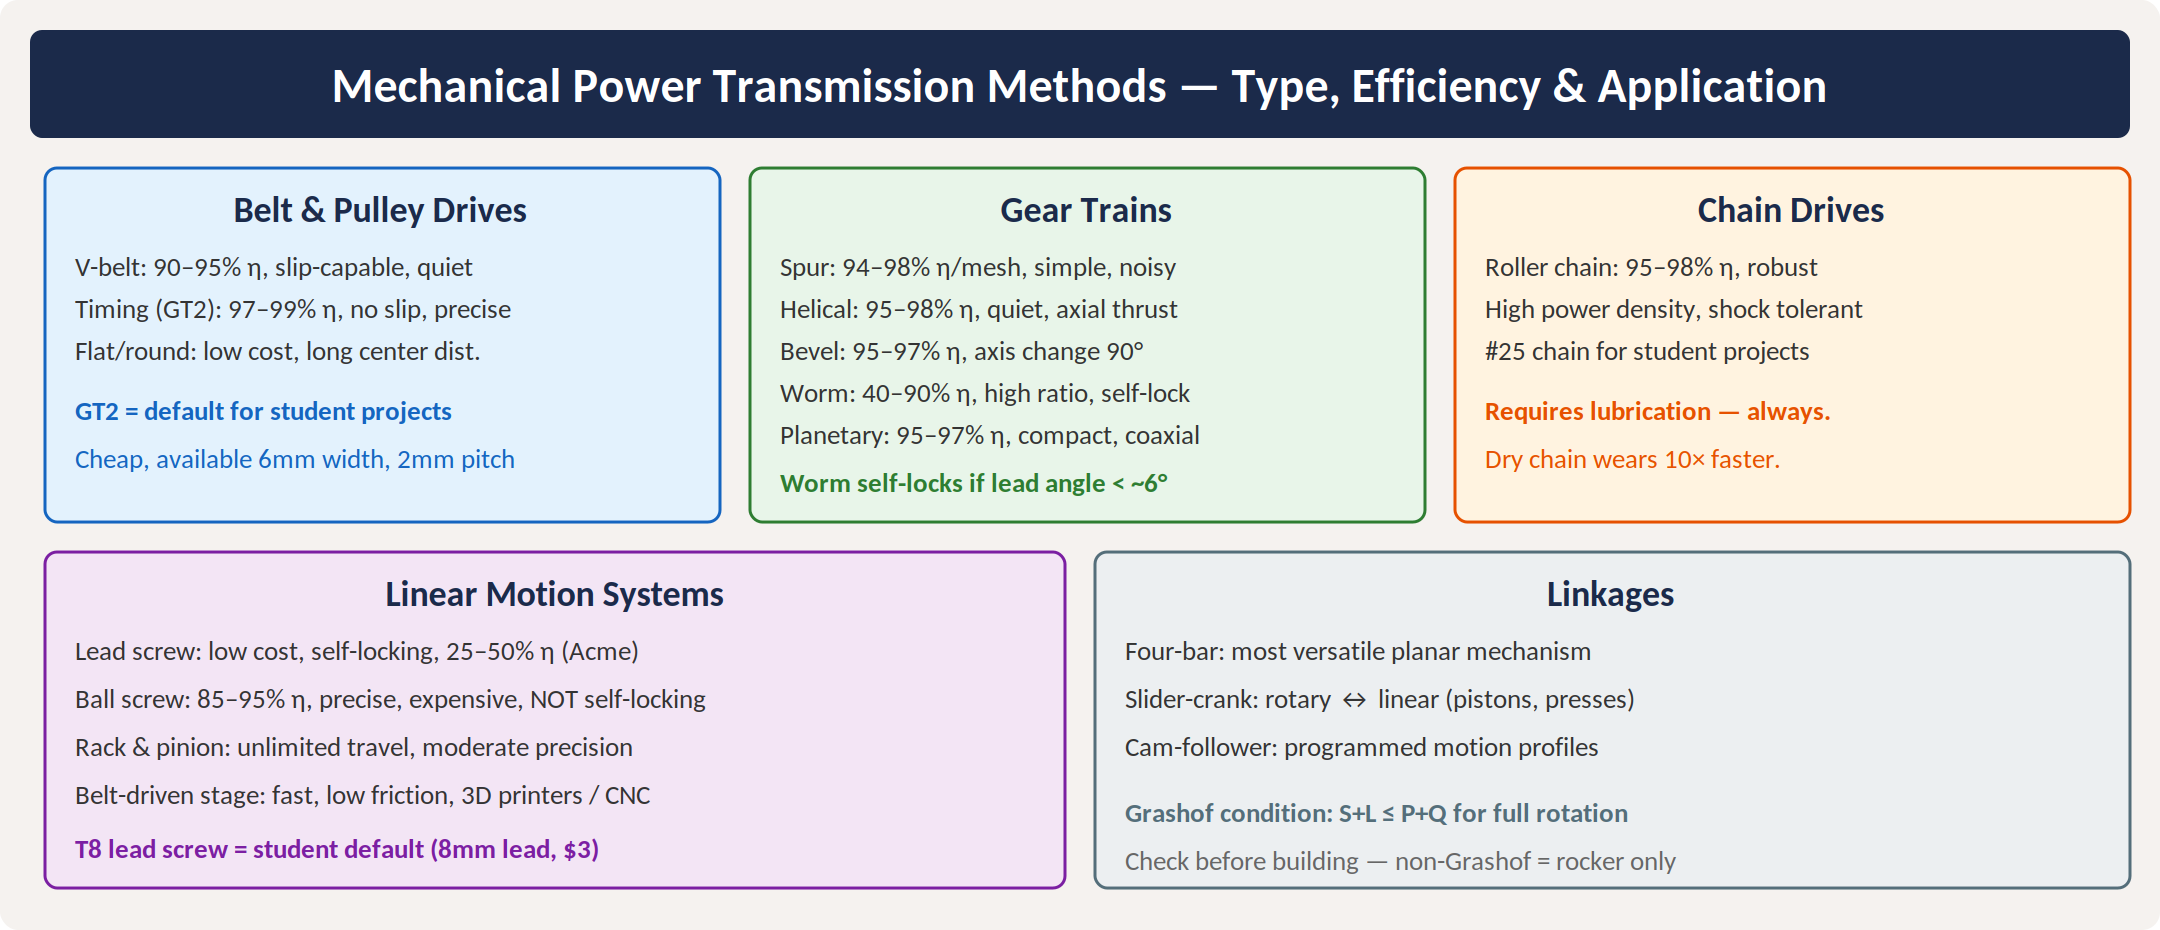
\includegraphics[width=\textwidth]{master_figs/fig_power_transmission_types.png}
\caption{Power transmission methods with efficiency, characteristics, and recommendations.}\label{fig:ptypes}
\end{figure}

\textbf{Spur}: straight teeth, 94--98\%/mesh, noisy at speed. \textbf{Helical}: angled teeth, quieter, generates axial thrust. \textbf{Bevel}: intersecting shafts (90$^{\circ}$). \textbf{Worm}: high ratio single-stage (5:1--100:1), 40--90\% efficient, \textbf{self-locking} when lead angle $<$$\sim$\ang{6}. \textbf{Planetary}: compact, coaxial, 95--97\%/stage.

\begin{tipbox}[Gear Selection for Student Projects]
ServoCity (servocity.com) sells matched spur gear\index{spur gear} sets with standardized shafts and hubs. McMaster has individual gears in any size. For 3D-printed gears: PETG or nylon, module $\geq$1.5, add 0.1--0.2\,mm backlash.
\end{tipbox}


\subsection{Gear Train Design Process}
\begin{enumerate}[nosep,leftmargin=1.5em]
\item Calculate required output torque and speed from the load.
\item Calculate gear ratio: $GR = \omega_{motor} / \omega_{load}$.
\item Select gear type based on noise, efficiency, and axis orientation requirements.
\item If $GR > 10$: use multi-stage (two spur stages) or single-stage worm/planetary.
\item Size gears for tooth bending stress and surface contact stress (Lewis equation for bending: $\sigma = W_t / (b \cdot m \cdot Y)$).
\item For student projects: select stock gears from ServoCity or McMaster and verify that the rated torque exceeds your load with $\geq$2$\times$ margin.
\item Specify mounting: shaft diameter, key or set screw, bearing supports, and housing.
\end{enumerate}

\subsection{Backlash and Precision}
Backlash is the angular play between mating gear teeth (or belt-pulley engagement). It causes positioning error and control-loop instability. Standard spur gears have 0.05--0.10\,mm backlash. For precision applications: use anti-backlash gears (split gear with spring preload), ball screws (inherently low backlash), or harmonic drives (zero backlash). For most MEGN~301 projects, standard backlash is acceptable.

\section{Shafts and Couplings}
\subsection{Shaft Design}
Shafts transmit torque and support rotating components. Default: 1045 steel. Size for torque with safety factor. Keyways add $\sim$25\% stress concentration.

\subsection{Shaft-Hub Connections}
\textbf{Keyway}: rectangular key transmits torque; standard sizes from ANSI B17.1. \textbf{Set screw}: clamps hub to flat; low torque, adequate for light student loads. \textbf{D-shaft}: flat on shaft engages matching hub flat; common on stepper motors.

\subsection{Couplings}
\textbf{Rigid}: zero misalignment tolerance. \textbf{Flexible}: jaw coupling (elastomer spider, shock absorption), beam coupling (zero backlash), Oldham (parallel offset), universal joint (large angles).

\section{Linear Motion}
\subsection{Lead Screws}
Acme-thread, 25--50\% efficient, \textbf{self-locking}. T8$\times$8 (8\,mm dia, 8\,mm lead) is the student default (\$3--8 with brass nut).

\subsection{Ball Screws}
Recirculating balls, 85--95\% efficient, precise, \textbf{not self-locking}. More expensive.

\subsection{Rack and Pinion}
Unlimited travel, moderate precision. Force = torque / pinion pitch radius.

\subsection{Belt-Driven Linear Stages}
Timing belt on two pulleys, carriage on linear rails. Fast, low friction. GT2 + MGN12 rail for student projects.

\section{Linkages}
\textbf{Four-bar}: most versatile planar mechanism. Grashof condition: $S + L \leq P + Q$ for full rotation. \textbf{Slider-crank}: rotary $\leftrightarrow$ linear (pistons, presses). Stroke = $2\times$ crank radius. \textbf{Cam-follower}: programmed motion profiles from cam shape.

\section{Selection Framework}
\begin{figure}[htbp]\centering
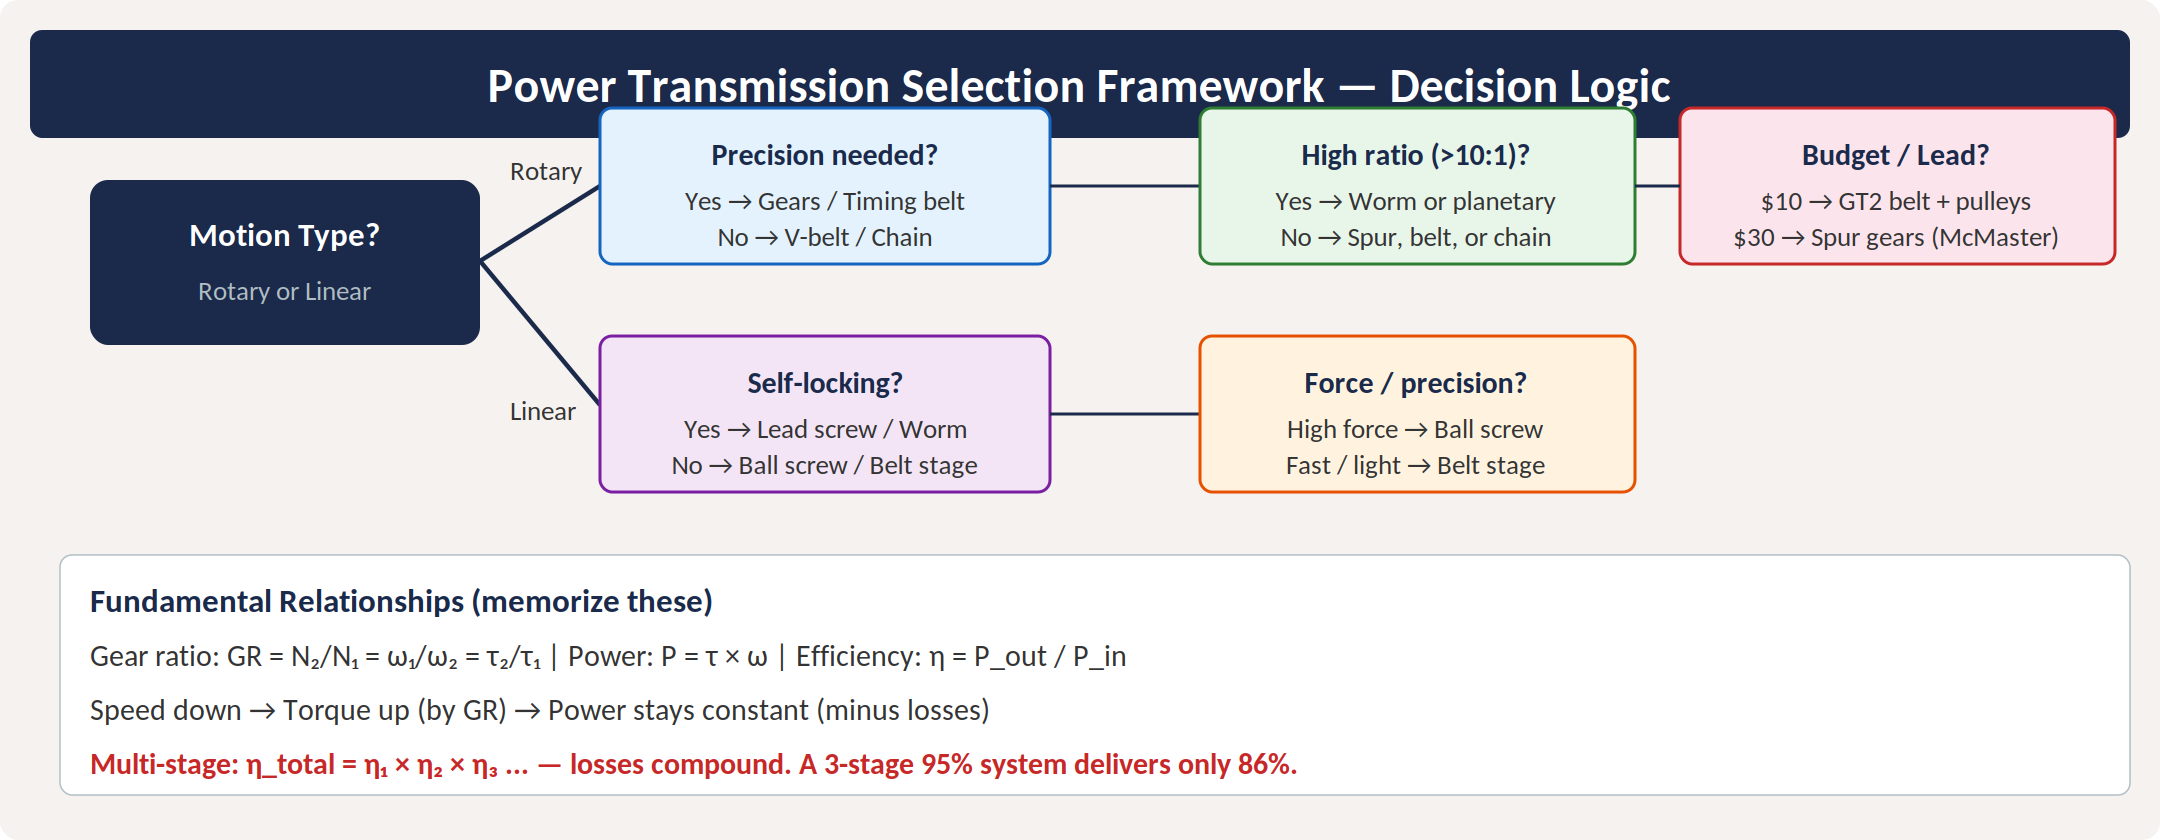
\includegraphics[width=\textwidth]{master_figs/fig_power_trans_selection.png}
\caption{Power transmission selection: motion type, precision, self-locking, ratio, budget.}\label{fig:ptsel}
\end{figure}

\begin{keyconceptbox}[Five Key Takeaways]
\begin{enumerate}[nosep,leftmargin=1.5em]
\item Speed down = torque up. Calculate output torque before selecting transmission.
\item GT2 belts and T8 lead screws are student defaults. Start there.
\item Efficiency compounds multiplicatively. Minimize stages.
\item Self-locking (lead screws, worms) holds position without power. Non-self-locking (ball screws, spur gears) needs a brake.
\item Every rotating joint needs a bearing. Every coupling needs defined misalignment tolerance.
\end{enumerate}
\end{keyconceptbox}


\begin{keyconceptbox}[Requirements Mapping: From Transmission Specs to Shall-Statements]
Power transmission design generates system requirements:
\begin{itemize}[nosep,leftmargin=1.5em]
\item ``Linear stage positions to $\pm$0.1\,mm'' $\to$ MECH-REQ: Lead screw shall have $\leq$0.05\,mm backlash. Anti-backlash nut required.
\item ``System holds position when unpowered'' $\to$ MECH-REQ: Transmission shall be self-locking (lead screw or worm gear\index{worm gear} with lead angle $<$\ang{6}).
\item ``Gear ratio 10:1 in minimum space'' $\to$ MECH-REQ: Use planetary gearbox ($\leq$40\,mm diameter) with $\geq$95\% efficiency per stage.
\end{itemize}
Calculate the required output torque and speed \emph{from requirements} before selecting any transmission hardware.
\end{keyconceptbox}

\section{Power Transmission Fundamentals}
Mechanical power transmission converts the motor's output (speed and torque at the motor shaft) into the required speed and torque at the load. The fundamental relationship:
\begin{equation}
P = T \cdot \omega
\end{equation}
where $P$ is power (W), $T$ is torque (N$\cdot$m), and $\omega$ is angular velocity (rad/s). Power is conserved (minus friction losses), so reducing speed increases torque proportionally: $T_{\text{out}} = T_{\text{in}} \times (N_{\text{in}}/N_{\text{out}}) \times \eta$ where $\eta$ is the efficiency.

\section{Belt and Chain Drives}
\textbf{Timing belts} (synchronous belts): positive engagement (no slip). Tooth profiles: GT2 (2\,mm pitch, standard for 3D printers and small mechanisms), HTD (higher torque capacity for larger systems). Advantages: precise speed ratio, no lubrication, quiet. Sizing: select belt width for the required torque; the belt manufacturer's catalog provides power ratings per unit width for each tooth profile.

\textbf{V-belts}: friction drive (slight slip under load). Simple, tolerant of misalignment, absorbs vibration. Used in industrial machinery, HVAC, and automotive accessories. Not suitable for precise positioning.

\textbf{Roller chain}: positive engagement, high torque capacity. Standard sizes: \#25 (1/4-inch pitch), \#35 (3/8-inch), \#40 (1/2-inch). Requires lubrication and tensioning. Noisy at high speed. Used in bicycles, motorcycles, and industrial conveyors.

\section{Lead Screws and Linear Motion}
Converting rotary motion to linear motion:

\textbf{Lead screws}: a threaded rod turns in a nut, translating rotary motion to linear motion. The lead $l$ (linear distance per revolution) determines the speed and force: $v = l \cdot n$ (speed), $F = 2\pi T/(l \cdot \eta)$ (force). Standard trapezoidal (ACME) thread: $\eta \approx 40\%$. Ball screws (recirculating ball bearings in the nut): $\eta \approx 90\%$, but 10$\times$ the cost.

\textbf{Rack and pinion}: a spur gear (pinion) meshes with a linear gear (rack). Linear speed $= \pi d n$ where $d$ is the pinion pitch diameter. Used in CNC machines, steering systems, and linear actuators.

\section{Coupling Selection}
Couplings connect two shafts and transmit torque. They must accommodate misalignment between the shafts:

\textbf{Rigid couplings}: no misalignment tolerance. Used only when shafts are precisely aligned (lathe spindles, precision instruments). Types: sleeve, clamp, keyed.

\textbf{Flexible couplings}: accommodate angular, parallel, and axial misalignment. Types: jaw (elastomer insert absorbs vibration; most common in student projects), beam (single-piece helical cut; allows angular and axial flex), Oldham (sliding disk; accommodates parallel offset), and universal joint (large angular misalignment for non-parallel shafts).

\textbf{Selection criteria}: (1) torque rating $\geq 2\times$ the maximum torque (safety factor for shock loads), (2) bore size matches both shafts, (3) misalignment tolerance $\geq$ the expected misalignment (typically $\pm$1\degC{} angular and $\pm$0.5\,mm parallel for student assemblies), (4) set screw or clamp style (clamp is preferred; set screws can loosen and damage the shaft).

\section{Efficiency and Heat Generation}
Every transmission element converts some input power to heat through friction. Typical efficiencies: spur gears 95--98\% per stage, timing belt 95--98\%, roller chain 95--98\%, V-belt 90--95\%, worm gear 40--90\% (depending on ratio), lead screw 30--50\% (ACME), ball screw 85--95\%.

For a two-stage spur gear train driving a lead screw: $\eta_{\text{total}} = 0.97 \times 0.97 \times 0.40 = 0.376$ (37.6\%). A 10\,W motor delivers only 3.76\,W to the load; 6.24\,W is dissipated as heat in the gear teeth and screw thread. This heat must be managed (lubrication, heat sinking, duty cycle limits) or the mechanism will overheat and seize.
\section{Gear Design for 3D-Printed Prototypes}
3D printing enables rapid prototyping of custom gears, but the material properties and dimensional accuracy impose limitations:

\textbf{FDM (PLA, ABS, PETG)}: layer lines on tooth flanks increase friction and noise. Typical tolerance: $\pm$0.2\,mm, which limits the minimum module to $m \geq 1.5$\,mm (smaller teeth do not print accurately). Tooth strength is limited by the layer adhesion (Z-direction strength is 30--70\% of XY strength). Print gears with teeth oriented in the XY plane for maximum strength. Expect 50--100 hours of operation before significant wear; suitable for proof-of-concept but not production.

\textbf{SLA (resin)}: much finer detail (tolerance $\pm$0.05\,mm), enabling module $\geq 0.5$\,mm. Smoother tooth surfaces reduce friction. However, standard SLA resins are brittle; use tough or engineering resins for functional gears. UV degradation limits outdoor use.

\textbf{Design tips}: (1) increase backlash to $1.5\times$ the standard value to accommodate print tolerance, (2) add a 0.5\,mm fillet at the tooth root to reduce stress concentration (which FDM's layer structure amplifies), (3) print a test gear pair and verify meshing before printing the full mechanism.

\section{Motor-to-Load Matching}
The motor must be selected to match the load's torque and speed requirements through the transmission. The design procedure:

\textbf{Step 1}: determine the load requirements at the output shaft. What torque ($T_{\text{load}}$) and speed ($n_{\text{load}}$) does the application need?

\textbf{Step 2}: select a gear ratio. $i = n_{\text{motor}}/n_{\text{load}}$. The motor's rated speed is typically 3000--12{,}000\,RPM; the load speed is often 10--500\,RPM.

\textbf{Step 3}: calculate the motor torque requirement. $T_{\text{motor}} = T_{\text{load}} / (i \times \eta)$ where $\eta$ is the transmission efficiency.

\textbf{Step 4}: select a motor whose rated torque exceeds $T_{\text{motor}}$ with a safety factor of $\geq 1.5$. Also verify that the motor's rated speed matches $n_{\text{load}} \times i$.

\textbf{Step 5}: verify the power. $P_{\text{motor}} = T_{\text{motor}} \times \omega_{\text{motor}} \geq T_{\text{load}} \times \omega_{\text{load}} / \eta$.

\begin{greenshieldbox}[GreenShield: Motor Selection for a Pump Drive]
The pump requires $T_{\text{load}} = 0.3$\,N$\cdot$m at $n_{\text{load}} = 300$\,RPM. Using a 2-stage spur gear reduction with $i = 10$ and $\eta = 0.94$: $T_{\text{motor}} = 0.3/(10 \times 0.94) = 0.032$\,N$\cdot$m at $n_{\text{motor}} = 3000$\,RPM. Power: $P = 0.3 \times 300 \times 2\pi/60 = 9.4$\,W. Select a motor rated for $\geq 0.048$\,N$\cdot$m (1.5$\times$ safety factor) at 3000\,RPM, with $\geq 15$\,W power rating. A typical 12\,V, 380-size brushed DC motor meets these requirements.
\end{greenshieldbox}

\section{Linear Actuator Design}
For applications requiring linear force (clamping, pressing, positioning), convert rotary motor output to linear motion:

\textbf{Lead screw actuator}: motor $\to$ coupling $\to$ lead screw $\to$ nut. Linear speed $v = l \times n$ (lead $\times$ RPM). Force $F = 2\pi T_{\text{motor}} \times i / l \times \eta$. Self-locking when the lead angle $< \arctan(\mu)$ (typically $< 5$\degC{}), meaning the load cannot back-drive the motor. This is useful for holding position without power.

\textbf{Belt-driven linear stage}: motor $\to$ timing pulley $\to$ belt $\to$ carriage. Linear speed $v = \pi d n$ (pulley diameter $\times$ RPM). Not self-locking; the carriage moves freely when the motor is unpowered (use a brake or worm gear if holding is needed). Very fast: typical belt-driven CNC axes achieve 200--500\,mm/s.

\textbf{Rack and pinion}: motor $\to$ pinion gear $\to$ rack. Linear speed $v = \pi d n$. Compact, high force, bidirectional. Common in CNC routers and industrial automation.

\section{Vibration and Noise in Power Transmission}
Gear noise arises from tooth meshing: each tooth engagement creates a brief impulse that excites structural resonances. Noise is proportional to speed, load, and gear quality. Mitigation: (1) use helical gears instead of spur (gradual engagement reduces impact), (2) increase gear quality grade (AGMA 8 or higher), (3) use plastic or composite gears for light loads (inherent damping reduces noise), (4) enclose the gear train in a housing with vibration-damping mounts.

Belt drives are inherently quieter than gears (flexible belt absorbs vibration). Chain drives are the noisiest (metal-on-metal impact at each link engagement). For noise-sensitive applications (laboratory instruments, medical devices, consumer products): use timing belts or direct drive (no transmission, oversized motor at the load speed).
\begin{keyconceptbox}[Requirements Mapping: Power Transmission]
\textbf{From technical specs to ``shall'' statements:}

A timing belt drive using a GT2 belt with a 20-tooth pulley ($d = 12.73$\,mm) at 3000\,RPM produces linear speed $v = \pi \times 0.01273 \times 3000/60 = 2.0$\,m/s. This becomes: ``SYS-SPD-001: The linear stage shall achieve a travel speed of $2.0 \pm 0.1$\,m/s. \emph{Verification: Test --- measure travel time over 500\,mm using a stopwatch ($N = 10$ trials).}''

A two-stage gear train ($i = 20$, $\eta = 0.94$) with a motor rated at 0.05\,N$\cdot$m delivers $0.05 \times 20 \times 0.94 = 0.94$\,N$\cdot$m at the output. This becomes: ``SYS-TRQ-001: The output shaft shall deliver $\geq 0.9$\,N$\cdot$m at 150\,RPM. \emph{Verification: Test --- measure stall torque with a spring scale at a known radius.}''
\end{keyconceptbox}

\begin{quickrefbox}[Quick Reference: Common Transmission Components for Student Projects]
\begin{table}[H]\centering\small
\begin{tabularx}{\textwidth}{l c c X}
\toprule
\textbf{Component} & \textbf{Spec} & \textbf{Source} & \textbf{Notes} \\
\midrule
GT2 belt (6\,mm) & 2\,mm pitch & Amazon, ServoCity & Standard for light linear stages \\
GT2 pulley (20T) & 5\,mm bore & Amazon, ServoCity & $d_{pitch} = 12.73$\,mm \\
T8$\times$8 lead screw & 8\,mm lead & Amazon & 26.7\,mm/s at 200\,RPM \\
T8$\times$2 lead screw & 2\,mm lead & Amazon, McMaster & 6.67\,mm/s at 200\,RPM; finer control \\
608 bearing (8\,mm ID) & ABEC-1 & McMaster, Amazon & Skate bearing; ubiquitous, cheap \\
6001 bearing (12\,mm ID) & ABEC-1 & McMaster & Common for NEMA 17 shafts \\
Oldham coupling & 5--8\,mm bore & ServoCity & Misalignment-tolerant shaft coupling \\
Flexible jaw coupling & 5--8\,mm bore & McMaster & Dampens vibration; easy install \\
\bottomrule
\end{tabularx}
\end{table}
\end{quickrefbox}

\section{Practice Questions}
\begin{enumerate}[leftmargin=1.5em]
\item A NEMA~17 stepper produces 0.4\,N$\cdot$m at 200\,RPM. You need 2.0\,N$\cdot$m at 40\,RPM. What gear ratio is required? What efficiency must the transmission achieve?
\item Compare GT2 timing belt vs.\ roller chain for a 3:1 reduction on a small conveyor. Which do you choose and why?
\item Your linear stage uses a T8$\times$8 lead screw driven by a stepper at 200\,RPM. Calculate the linear speed in mm/s. If the stage must move 200\,mm, how long does the motion take?
\item A worm gear set has a 30:1 ratio and 60\% efficiency. Input power is 50\,W. What is the output power? Is this set self-locking?
\item Your project needs a mechanism that converts continuous motor rotation into a back-and-forth linear stroke of 50\,mm. Propose two different mechanism solutions and compare them.
\item A 4-bar linkage has link lengths 40, 100, 70, and 80\,mm. Check the Grashof condition. Which link(s) can make a full revolution?
\item Your belt-driven linear stage stalls under load. The stepper motor skips steps but does not overheat. Diagnose the root cause and propose fixes.
\end{enumerate}

\subsection{Answers}
\begin{enumerate}[leftmargin=1.5em]
\item $GR = 2.0/0.4 = 5:1$ (or $200/40 = 5:1$). Check: $P_{in} = 0.4 \times (200 \times 2\pi/60) = 8.38$\,W. $P_{out} = 2.0 \times (40 \times 2\pi/60) = 8.38$\,W for 100\% efficiency. With real losses, the transmission must be $\geq$100\% to deliver full torque; meaning the motor is marginally sized. Derate: need $\geq$85\% efficient transmission (GT2 belt: 97\%, spur gear: 94\% work; worm at 60\% does not).
\item GT2 belt: no lubrication, clean, quiet, 97\% efficient, \$10 total. Chain: requires lube, messy, noisier, 96\% efficient, \$15. For a small indoor conveyor, GT2 wins on cleanliness, cost, and simplicity. Chain is better if the conveyor sees high shock loads or outdoor contamination.
\item Linear speed = lead $\times$ RPM / 60 = 8\,mm $\times$ 200/60 = 26.7\,mm/s. Time = 200/26.7 = 7.5\,s.
\item $P_{out} = 50 \times 0.60 = 30$\,W. At 30:1 ratio, the lead angle is very low ($\ll$\ang{6}), so yes; self-locking.
\item (a) Slider-crank: crank radius = 25\,mm, continuous rotation $\to$ 50\,mm stroke. Simple, constant stroke. (b) Belt-driven stage with limit switches: motor reverses at each end. Variable stroke and speed via firmware. Slider-crank is simpler mechanically; belt stage is more flexible.
\item $S = 40, L = 100, P = 70, Q = 80$. $S + L = 140$. $P + Q = 150$. $140 \leq 150$. Grashof satisfied. The shortest link (40\,mm) can make full revolution. If grounded, it is the crank.
\item Motor torque is sufficient (no overheating) but the belt/pulley system cannot transmit the load. Causes: belt tension too low (belt slips on pulley teeth), pulley set screw loose (pulley spins on shaft), or load exceeds belt rating. Fixes: increase belt tension, verify set screws, check that belt width and tooth count match the load.
\end{enumerate}

